% Options for packages loaded elsewhere
\PassOptionsToPackage{unicode}{hyperref}
\PassOptionsToPackage{hyphens}{url}
%
\documentclass[
  ignorenonframetext,
]{beamer}
\usepackage{pgfpages}
\setbeamertemplate{caption}[numbered]
\setbeamertemplate{caption label separator}{: }
\setbeamercolor{caption name}{fg=normal text.fg}
\beamertemplatenavigationsymbolsempty
% Prevent slide breaks in the middle of a paragraph
\widowpenalties 1 10000
\raggedbottom
\setbeamertemplate{part page}{
  \centering
  \begin{beamercolorbox}[sep=16pt,center]{part title}
    \usebeamerfont{part title}\insertpart\par
  \end{beamercolorbox}
}
\setbeamertemplate{section page}{
  \centering
  \begin{beamercolorbox}[sep=12pt,center]{part title}
    \usebeamerfont{section title}\insertsection\par
  \end{beamercolorbox}
}
\setbeamertemplate{subsection page}{
  \centering
  \begin{beamercolorbox}[sep=8pt,center]{part title}
    \usebeamerfont{subsection title}\insertsubsection\par
  \end{beamercolorbox}
}
\AtBeginPart{
  \frame{\partpage}
}
\AtBeginSection{
  \ifbibliography
  \else
    \frame{\sectionpage}
  \fi
}
\AtBeginSubsection{
  \frame{\subsectionpage}
}
\usepackage{lmodern}
\usepackage{amssymb,amsmath}
\usepackage{ifxetex,ifluatex}
\ifnum 0\ifxetex 1\fi\ifluatex 1\fi=0 % if pdftex
  \usepackage[T1]{fontenc}
  \usepackage[utf8]{inputenc}
  \usepackage{textcomp} % provide euro and other symbols
\else % if luatex or xetex
  \usepackage{unicode-math}
  \defaultfontfeatures{Scale=MatchLowercase}
  \defaultfontfeatures[\rmfamily]{Ligatures=TeX,Scale=1}
\fi
% Use upquote if available, for straight quotes in verbatim environments
\IfFileExists{upquote.sty}{\usepackage{upquote}}{}
\IfFileExists{microtype.sty}{% use microtype if available
  \usepackage[]{microtype}
  \UseMicrotypeSet[protrusion]{basicmath} % disable protrusion for tt fonts
}{}
\makeatletter
\@ifundefined{KOMAClassName}{% if non-KOMA class
  \IfFileExists{parskip.sty}{%
    \usepackage{parskip}
  }{% else
    \setlength{\parindent}{0pt}
    \setlength{\parskip}{6pt plus 2pt minus 1pt}}
}{% if KOMA class
  \KOMAoptions{parskip=half}}
\makeatother
\usepackage{xcolor}
\IfFileExists{xurl.sty}{\usepackage{xurl}}{} % add URL line breaks if available
\IfFileExists{bookmark.sty}{\usepackage{bookmark}}{\usepackage{hyperref}}
\hypersetup{
  pdftitle={MA8701 Advanced methods in statistical inference and learning},
  pdfauthor={Mette Langaas IMF/NTNU},
  hidelinks,
  pdfcreator={LaTeX via pandoc}}
\urlstyle{same} % disable monospaced font for URLs
\newif\ifbibliography
\usepackage{color}
\usepackage{fancyvrb}
\newcommand{\VerbBar}{|}
\newcommand{\VERB}{\Verb[commandchars=\\\{\}]}
\DefineVerbatimEnvironment{Highlighting}{Verbatim}{commandchars=\\\{\}}
% Add ',fontsize=\small' for more characters per line
\usepackage{framed}
\definecolor{shadecolor}{RGB}{248,248,248}
\newenvironment{Shaded}{\begin{snugshade}}{\end{snugshade}}
\newcommand{\AlertTok}[1]{\textcolor[rgb]{0.94,0.16,0.16}{#1}}
\newcommand{\AnnotationTok}[1]{\textcolor[rgb]{0.56,0.35,0.01}{\textbf{\textit{#1}}}}
\newcommand{\AttributeTok}[1]{\textcolor[rgb]{0.77,0.63,0.00}{#1}}
\newcommand{\BaseNTok}[1]{\textcolor[rgb]{0.00,0.00,0.81}{#1}}
\newcommand{\BuiltInTok}[1]{#1}
\newcommand{\CharTok}[1]{\textcolor[rgb]{0.31,0.60,0.02}{#1}}
\newcommand{\CommentTok}[1]{\textcolor[rgb]{0.56,0.35,0.01}{\textit{#1}}}
\newcommand{\CommentVarTok}[1]{\textcolor[rgb]{0.56,0.35,0.01}{\textbf{\textit{#1}}}}
\newcommand{\ConstantTok}[1]{\textcolor[rgb]{0.00,0.00,0.00}{#1}}
\newcommand{\ControlFlowTok}[1]{\textcolor[rgb]{0.13,0.29,0.53}{\textbf{#1}}}
\newcommand{\DataTypeTok}[1]{\textcolor[rgb]{0.13,0.29,0.53}{#1}}
\newcommand{\DecValTok}[1]{\textcolor[rgb]{0.00,0.00,0.81}{#1}}
\newcommand{\DocumentationTok}[1]{\textcolor[rgb]{0.56,0.35,0.01}{\textbf{\textit{#1}}}}
\newcommand{\ErrorTok}[1]{\textcolor[rgb]{0.64,0.00,0.00}{\textbf{#1}}}
\newcommand{\ExtensionTok}[1]{#1}
\newcommand{\FloatTok}[1]{\textcolor[rgb]{0.00,0.00,0.81}{#1}}
\newcommand{\FunctionTok}[1]{\textcolor[rgb]{0.00,0.00,0.00}{#1}}
\newcommand{\ImportTok}[1]{#1}
\newcommand{\InformationTok}[1]{\textcolor[rgb]{0.56,0.35,0.01}{\textbf{\textit{#1}}}}
\newcommand{\KeywordTok}[1]{\textcolor[rgb]{0.13,0.29,0.53}{\textbf{#1}}}
\newcommand{\NormalTok}[1]{#1}
\newcommand{\OperatorTok}[1]{\textcolor[rgb]{0.81,0.36,0.00}{\textbf{#1}}}
\newcommand{\OtherTok}[1]{\textcolor[rgb]{0.56,0.35,0.01}{#1}}
\newcommand{\PreprocessorTok}[1]{\textcolor[rgb]{0.56,0.35,0.01}{\textit{#1}}}
\newcommand{\RegionMarkerTok}[1]{#1}
\newcommand{\SpecialCharTok}[1]{\textcolor[rgb]{0.00,0.00,0.00}{#1}}
\newcommand{\SpecialStringTok}[1]{\textcolor[rgb]{0.31,0.60,0.02}{#1}}
\newcommand{\StringTok}[1]{\textcolor[rgb]{0.31,0.60,0.02}{#1}}
\newcommand{\VariableTok}[1]{\textcolor[rgb]{0.00,0.00,0.00}{#1}}
\newcommand{\VerbatimStringTok}[1]{\textcolor[rgb]{0.31,0.60,0.02}{#1}}
\newcommand{\WarningTok}[1]{\textcolor[rgb]{0.56,0.35,0.01}{\textbf{\textit{#1}}}}
\usepackage{longtable,booktabs}
\usepackage{caption}
% Make caption package work with longtable
\makeatletter
\def\fnum@table{\tablename~\thetable}
\makeatother
\usepackage{graphicx,grffile}
\makeatletter
\def\maxwidth{\ifdim\Gin@nat@width>\linewidth\linewidth\else\Gin@nat@width\fi}
\def\maxheight{\ifdim\Gin@nat@height>\textheight\textheight\else\Gin@nat@height\fi}
\makeatother
% Scale images if necessary, so that they will not overflow the page
% margins by default, and it is still possible to overwrite the defaults
% using explicit options in \includegraphics[width, height, ...]{}
\setkeys{Gin}{width=\maxwidth,height=\maxheight,keepaspectratio}
% Set default figure placement to htbp
\makeatletter
\def\fps@figure{htbp}
\makeatother
\setlength{\emergencystretch}{3em} % prevent overfull lines
\providecommand{\tightlist}{%
  \setlength{\itemsep}{0pt}\setlength{\parskip}{0pt}}
\setcounter{secnumdepth}{-\maxdimen} % remove section numbering

\title{MA8701 Advanced methods in statistical inference and learning}
\subtitle{L4: Statistical inference}
\author{Mette Langaas IMF/NTNU}
\date{31 January, 2021}

\begin{document}
\frame{\titlepage}

\begin{frame}{Shrinkage - third act}
\protect\hypertarget{shrinkage---third-act}{}

\begin{block}{Outline}

\begin{itemize}
\tightlist
\item
  South African heart disease: classification with two classes,
  understand print-out from glm and glmnet, and inference with CI and
  \(p\)-values
\item
  Prediction vs statistics inference: what are the aims? Sampling
  distributions
\item
  Bayesian lasso
\item
  Boostrapping
\item
  Sample splitting
\item
  Inference after selection (Forward regression example, Polyhedral
  result, PoSI)
\item
  Reproducibility crisis and selective inference
\end{itemize}

\end{block}

\end{frame}

\begin{frame}

\begin{block}{Literature L4}

\textbf{Main source:}

\begin{itemize}
\tightlist
\item
  {[}HTW{]} Hastie, Tibshirani, Wainwrigh: ``Statistical Learning with
  Sparsity: The Lasso and Generalizations''. CRC press.
  \href{https://trevorhastie.github.io/}{Ebook}. Chapter 6.0, 6.1, 6.2,
  6.5. (Mention some results from 6.3 and 6.4.)
\end{itemize}

\textbf{Supplemental sources:}

\begin{itemize}
\item
  \href{https://www.math.ntnu.no/emner/TMA4267/2017v/multtest.pdf}{Short
  note on multiple hypothesis testing} in TMA4267 Linear Statistical
  Models, Kari K. Halle, Øyvind Bakke and Mette Langaas, March 15, 2017.
\item
  Single/multi-sampling splitting part of
  \href{https://projecteuclid.org/download/pdfview_1/euclid.ss/1449670857}{Dezeure,
  Bühlmann, Meier, Meinshausen (2015)}. ``High-Dimensional Inference:
  Confidence Intervals, p-Values and R-Software hdi''. Statistical
  Science, 2015, Vol. 30, No.~4, 533--558 DOI: 10.1214/15-STS527 (only
  the single/multiple sample splitting part in 2.1.1 and 2.2 for linear
  regression, and using the method in practice).
\item
  \href{https://www.pnas.org/content/112/25/7629}{Taylor and Tibshirani
  (2015)}: Statistical learning and selective inference, PNAS, vol 112,
  no 25, pages 7629-7634. (Soft version of HTW 6.3.2)
\end{itemize}

\end{block}

\end{frame}

\begin{frame}{South African heart disease}
\protect\hypertarget{south-african-heart-disease}{}

We start by discussing the data analysis included in the class material
from L3, but not discussed in class before.

\href{http://htmlpreview.github.io/?https://github.com/mettelang/MA8701V2021/blob/main/Part1/L3.html\#Example:_South_African_heart_disease}{L3
South African heart disease}

\textbf{Group discussion:}

\begin{itemize}
\tightlist
\item
  What is done?
\item
  What are the results?
\item
  Where are the confidence intervals and \(p\)-values in the ridge and
  lasso print-out?
\end{itemize}

\end{frame}

\begin{frame}

\begin{block}{Confidence interval}

\textbf{Set-up}

\begin{itemize}
\tightlist
\item
  We have a random sample \(Y_1,Y_2,\ldots,Y_N\) from
\item
  some distribution \(F\) with some (unkonwn) parameter \(\theta\).
\item
  Let \(y_1,y_2,\ldots,y_N\) be the observed values for the random
  sample.
\end{itemize}

\textbf{Statistics}

\begin{itemize}
\tightlist
\item
  We have two statistics \(\hat{\theta}_L(Y_1,Y_2,\ldots,Y_N)\) and
  \(\hat{\theta}_U(Y_1,Y_2,\ldots,Y_N)\) so that
\end{itemize}

\[P(\hat{\theta}_L(Y_1,Y_2,\ldots,Y_N)\le \theta \le \hat{\theta}_U(Y_1,Y_2,\ldots,Y_N))=1-\alpha\]
where \(\alpha\in [0,1]\)

\textbf{Confidence interval}

The numerical interval
\[[\hat{\theta}_L(y_1,y_2,\ldots,y_N),\hat{\theta}_U(y_1,y_2,\ldots,y_N)]\]
is called a \((1-\alpha)\) 100\% confidence interval.

\end{block}

\end{frame}

\begin{frame}

\begin{block}{Single hypothesis test}

\[H_{0}\colon \beta_j=0 \hspace{0.5cm} \text{vs.} \hspace{0.5cm} H_{1}\colon \beta_j \neq 0\]

\begin{longtable}[]{@{}lll@{}}
\toprule
& Not reject \(H_0\) & Reject \(H_0\)\tabularnewline
\midrule
\endhead
\(H_0\) true & Correct & Type I error\tabularnewline
\(H_0\) false & Type II error & Correct\tabularnewline
\bottomrule
\end{longtable}

\end{block}

\end{frame}

\begin{frame}

\begin{itemize}
\tightlist
\item
  Two types of errors are possible, type I error and type II error.
\item
  A type I error would be to reject \(H_0\) when \(H_0\) is true, that
  is concluding that there is a linear association between the response
  and the predictor where there is no such association. This is called a
  \emph{false positive finding}.
\item
  A type II error would be to fail to reject \(H_0\) when the
  alternative hypothesis \(H_1\) is true, that is not detecting that
  there is a linear association between the response and the covariate.
  This is called a \emph{false negative finding}.
\end{itemize}

\end{frame}

\begin{frame}

\begin{block}{\(p\)-value}

\begin{itemize}
\tightlist
\item
  A \(p\)-value \(p(X)\) is a test statistic satisfying
  \(0 \leq p({\bf Y}) \leq 1\) for every vector of observations
  \(\bf{Y}\).
\item
  Small values give evidence that \(H_1\) is true.
\item
  In single hypothesis testing, if the \(p\)-value is less than the
  chosen significance level (chosen upper limit for the probability of
  committing a type I error), then we reject the null hypothesis,
  \(H_0\).
\item
  The chosen significance level is often referred to as \(\alpha\).
\end{itemize}

\end{block}

\end{frame}

\begin{frame}

A \(p\)-value is \emph{valid} if
\[ P(p(\bf{Y}) \leq \alpha) \leq \alpha \] for all \(\alpha\),
\(0 \leq \alpha \leq 1\), whenever \(H_0\) is true, that is, if the
\(p\)-value is valid, rejection on the basis of the \(p\)-value ensures
that the probability of type I error does not exceed \(\alpha\).

\end{frame}

\begin{frame}

An \emph{exact} \(p\)-value satisfies
\[P(p(\bf{Y}) \leq \alpha) = \alpha\] for all \(\alpha\),
\(0 \leq \alpha \leq 1\).

\begin{itemize}
\tightlist
\item
  The exact \(p\)-value is uniformly distributed when the null
  hypothesis is true.
\item
  This is a fact that is often misunderstood by users of \(p\)-values.
\item
  The incorrect urban myth is that \(p\)-values from true null
  hypotheses are close to one, when the correct fact is that all values
  in intervals of the same length are equally probable (which is a
  property of the uniform distribution).
\end{itemize}

\end{frame}

\begin{frame}{Statistical inference}
\protect\hypertarget{statistical-inference}{}

We have now heard about the South African heart disease data, and we
will also look at at a regression problem with prediction of disease
progression in diabetes.

\end{frame}

\begin{frame}[fragile]

\begin{block}{Diabetes data}

In a medical study the aim was to explain the ethiology of diabetes
progression. Data was collected from \(n=442\) diabetes patients, and
from each patient the following measurements are available:

\begin{itemize}
\tightlist
\item
  \texttt{age} (in years) at baseline
\item
  \texttt{sex} (0=female and 1=male) at baseline
\item
  body mass index (\texttt{bmi}) at baseline
\item
  mean arterial blood pressure (\texttt{map}) at baseline
\item
  six blood serum measurements: total cholesterol (\texttt{tc}), ldl
  cholesterol (\texttt{ldl}), hdl cholesterol (\texttt{hdl}),
  \texttt{tch}, \texttt{ltg}, glucose \texttt{glu}, all at baseline,
\item
  a quantitative measurement of disease progression one year after
  baseline (\texttt{prog})
\end{itemize}

All measurements except \texttt{sex} are continuous. There are 10
covariates.

The response is the disease progression \texttt{prog} - thus a
regression problem.

\end{block}

\end{frame}

\begin{frame}[fragile]

Data can be

\begin{itemize}
\tightlist
\item
  downloaded from
  \url{https://web.stanford.edu/~hastie/StatLearnSparsity_files/DATA/diabetes.html}
  in three variants: raw, standardized and 442 \(\times\) 64 matrix with
  quadratic terms (not used here).
\item
  Or, loaded from the \texttt{lars} package, that is automatically
  loaded in the \texttt{monomvn} package (where \texttt{blasso} is
  found).
\end{itemize}

\end{frame}

\begin{frame}

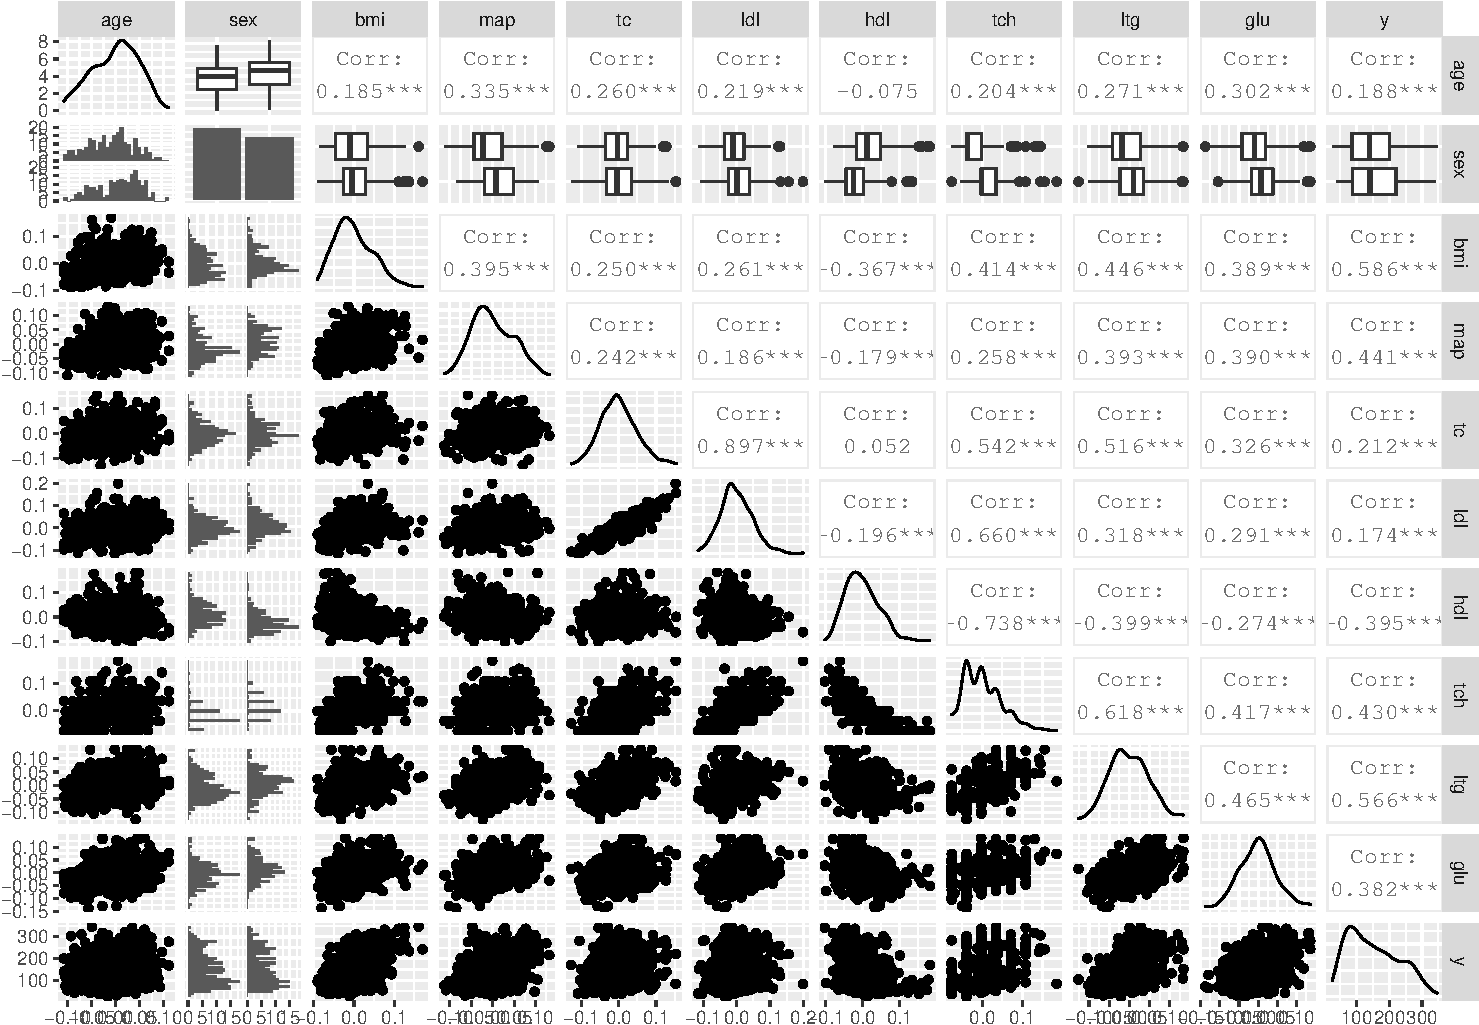
\includegraphics{L4_files/figure-beamer/unnamed-chunk-1-1.pdf}

\end{frame}

\begin{frame}

\begin{block}{Prediction vs statistical inference}

\begin{block}{Prediction}

\begin{itemize}
\tightlist
\item
  Predict the value of the progression variable for a person with
  diabetes.
\item
  Predict the probability of heart disease for a person from the
  population in the South African heart disease example.
\end{itemize}

\end{block}

\begin{block}{Inference}

\begin{itemize}
\tightlist
\item
  Assess the goodness of the prediction (MSE, error rate, ROC-AUC) -
  with uncertainty.
\item
  Interpret the GLM-model - which covariates is included?
\item
  Confidence interval for the model regression parameters.
\item
  Testing hypotheses about the model regression parameters.
\end{itemize}

\end{block}

\end{block}

\end{frame}

\begin{frame}

\begin{block}{Statistics vs Machine learning}

Figures redrawn from {[}Robert Tibshiran´s Breiman lecture at the NIPS
2015{]} (\url{https://www.youtube.com/watch?v=RKQJEvc02hc\&t=81s}).
(Conference on Neural Information Processing System)

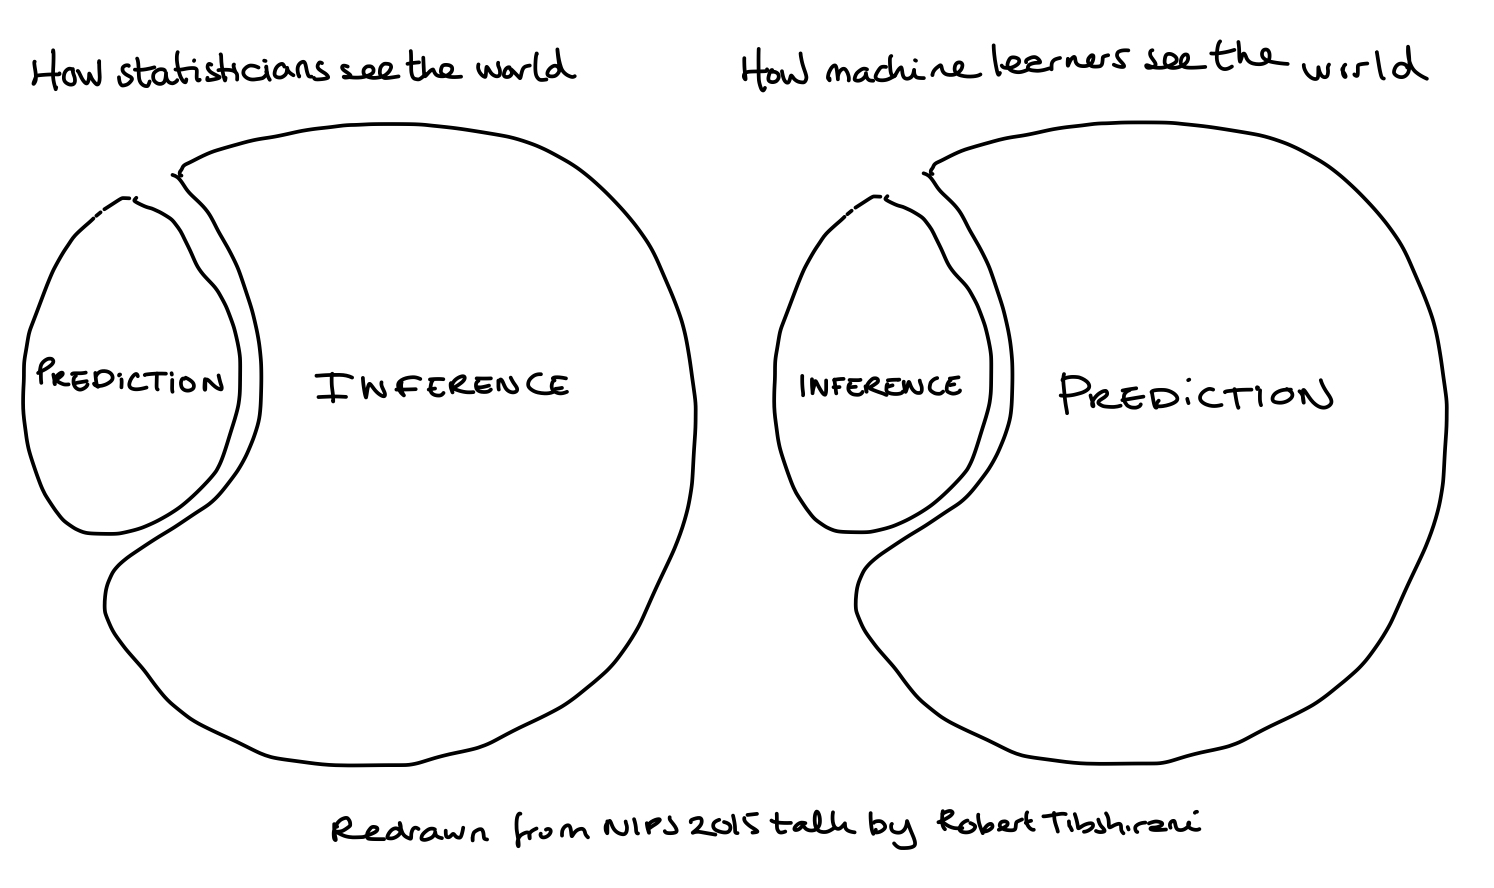
\includegraphics[width=0.7\linewidth]{./StatsvsMLPredInf}

\end{block}

\end{frame}

\begin{frame}

\begin{block}{Known sampling distributions}

For the linear regression and logistic regression we know the sampling
distribution of the regression coefficient estimators.

Then it is easy to construct confidence intervals and perform hypothesis
tests.

What are the known results?

\end{block}

\end{frame}

\begin{frame}

\end{frame}

\begin{frame}

\begin{block}{Sampling distribution for ridge and lasso?}

\begin{block}{Ridge}

From L2: for the normal linear model

\[ \hat{\beta}_{\text{ridge}}=({\bf X}^T{\bf X}+\lambda {\bf I})^{-1} {\bf X}^T {\bf Y}\]

\[\hat{\beta}(\lambda)_{\text{ridge}} \sim N \{ (\mathbf{X}^T \mathbf{X} + \lambda \mathbf{I}_{p})^{-1} \mathbf{X}^T \mathbf{X} \, \beta,\]

\[\sigma^2 ( \mathbf{X}^T \mathbf{X} + \lambda \mathbf{I}_{p} )^{-1}  \mathbf{X}^T \mathbf{X} ( \mathbf{X}^T \mathbf{X} + \lambda \mathbf{I}_{p} )^{-1}  \}.\]

\[\text{df}(\lambda)=\text{tr}({\bf H}_{\lambda})=\text{tr}({\bf X}({\bf X}^T{\bf X}+ \lambda {\bf I})^{-1}{\bf X}^T)=\cdots=\sum_{j=1}^p \frac{d_j^2}{d_j^2+\lambda}\]
What can we do with that?

\end{block}

\end{block}

\end{frame}

\begin{frame}

\end{frame}

\begin{frame}

\begin{block}{Lasso}

Some results using approximations to ridge (for mean and variance, see
WNvW p 97), but else \emph{no parametric version of sampling
distribution} known.

\end{block}

\end{frame}

\begin{frame}

\begin{block}{Conclusion}

This is absolutely not straight forward.

The \emph{adaptive nature} of the estimation procedures makes it
challenging to perform inference.

\begin{itemize}
\tightlist
\item
  We will \emph{discuss} possible solutions to finding confidence
  intervals for regression parameters for lasso, and for constructing
  \(p\)-values for testing hypotheses about the regression parameters.
\item
  We will address some \emph{philosophical principles behind inference}
\item
  and mention topics that can be studied further for the interested
  student!
\end{itemize}

Warning: there seems not to be consensus, but many interesting
approaches and ideas that we may consider.

\end{block}

\end{frame}

\begin{frame}{Bayesian lasso}
\protect\hypertarget{bayesian-lasso}{}

(HTW 6.1)

In the Bayesian statistics the regression parameters \(\beta\) are
random quantities, and in addition to the likelihood also a prior for
the regression parameters (and other parameters) are needed.

Multiple linear regression: distribution of response - where we for
simplicity assume that we have centred covariates and centred response
(so no intercept term)

\[ {\bf y}\mid \beta, \lambda, \sigma \sim N({\bf X}\beta,\sigma^2 {\bf I})\]

Prior for regression parameters

\[\beta \mid \lambda, \sigma \sim \prod_{j=1}^p \frac{\lambda}{2 \sigma}\exp(-\frac{\lambda}{\sigma}\lvert \beta_j \rvert)\]

This prior is called an i.i.d. \emph{Laplacian} (or double exponential)
prior.

\end{frame}

\begin{frame}

It can be shown that the negative log of the posterior density for
\(\beta \mid {\bf y}, \lambda, \sigma\) is (up to an additive constant)

\[\frac{1}{2\sigma^2} \Vert {\bf y}-{\bf X}\beta\Vert_2^2 +\frac{\lambda}{\sigma} \Vert \beta \Vert_1\]

Does this look familiar?

\end{frame}

\begin{frame}

For a fixed value of \(\sigma\) and \(\lambda\) - the \(\beta\) giving
the minimum of the negative log posterior is the \emph{lasso} estimate
where the regularization parameter is \(\sigma \lambda\).

The minimum negative log posterior will then be the same as the maximum
log posterior - and the maximum of a distribution is called the
\emph{mode} of the distribution.

The lasso estimate is the posterior mode in the Bayesian model.

(Study Figure 6.1 in HTW: describe what we see.)

\end{frame}

\begin{frame}

(Study Figure 6.2 in HTW: compares lasso path with Bayesian lasso with
different \(\lambda\)s.)

A full Bayesian approach requires priors for \(\lambda\) and \(\sigma\)
also.

Markov Chain Monte Carlo MCMC is used efficiently sample realizations
form the posterior distribution.

\end{frame}

\begin{frame}

\begin{block}{Not only the point estimate}

The posterior distribution gives the

\begin{itemize}
\tightlist
\item
  point estimates for the lasso (the mode of the distribution)
\end{itemize}

but

\begin{itemize}
\tightlist
\item
  also the \emph{entire joint distribution}.
\end{itemize}

(Study Figure 6.3 in HTW for boxplots and marginal density one
regression parameter - based on a \emph{sample} from the posterior
distribution.)

\end{block}

\end{frame}

\begin{frame}[fragile]

\begin{block}{Diabetes example with \texttt{blasso}}

\begin{Shaded}
\begin{Highlighting}[]
\CommentTok{## code below copied from the help(blasso)}
\CommentTok{## following the lars diabetes example}
\KeywordTok{data}\NormalTok{(diabetes)}
\KeywordTok{attach}\NormalTok{(diabetes)}

\CommentTok{## Ordinary Least Squares regression}
\NormalTok{reg.ols <-}\StringTok{ }\KeywordTok{regress}\NormalTok{(x, y)}

\CommentTok{## Lasso regression}
\NormalTok{reg.las <-}\StringTok{ }\KeywordTok{regress}\NormalTok{(x, y, }\DataTypeTok{method=}\StringTok{"lasso"}\NormalTok{)}

\CommentTok{## Bayesian Lasso regression}
\NormalTok{reg.blas <-}\StringTok{ }\KeywordTok{blasso}\NormalTok{(x, y,}\DataTypeTok{verb=}\DecValTok{0}\NormalTok{)}

\CommentTok{## summarize the beta (regression coefficients) estimates}
\KeywordTok{plot}\NormalTok{(reg.blas, }\DataTypeTok{burnin=}\DecValTok{200}\NormalTok{)}
\KeywordTok{points}\NormalTok{(}\KeywordTok{drop}\NormalTok{(reg.las}\OperatorTok{$}\NormalTok{b), }\DataTypeTok{col=}\DecValTok{2}\NormalTok{, }\DataTypeTok{pch=}\DecValTok{20}\NormalTok{)}
\KeywordTok{points}\NormalTok{(}\KeywordTok{drop}\NormalTok{(reg.ols}\OperatorTok{$}\NormalTok{b), }\DataTypeTok{col=}\DecValTok{3}\NormalTok{, }\DataTypeTok{pch=}\DecValTok{18}\NormalTok{)}
\KeywordTok{legend}\NormalTok{(}\StringTok{"topleft"}\NormalTok{, }\KeywordTok{c}\NormalTok{(}\StringTok{"blasso-map"}\NormalTok{, }\StringTok{"lasso"}\NormalTok{, }\StringTok{"lsr"}\NormalTok{),}
       \DataTypeTok{col=}\KeywordTok{c}\NormalTok{(}\DecValTok{2}\NormalTok{,}\DecValTok{2}\NormalTok{,}\DecValTok{3}\NormalTok{), }\DataTypeTok{pch=}\KeywordTok{c}\NormalTok{(}\DecValTok{21}\NormalTok{,}\DecValTok{20}\NormalTok{,}\DecValTok{18}\NormalTok{))}
\end{Highlighting}
\end{Shaded}

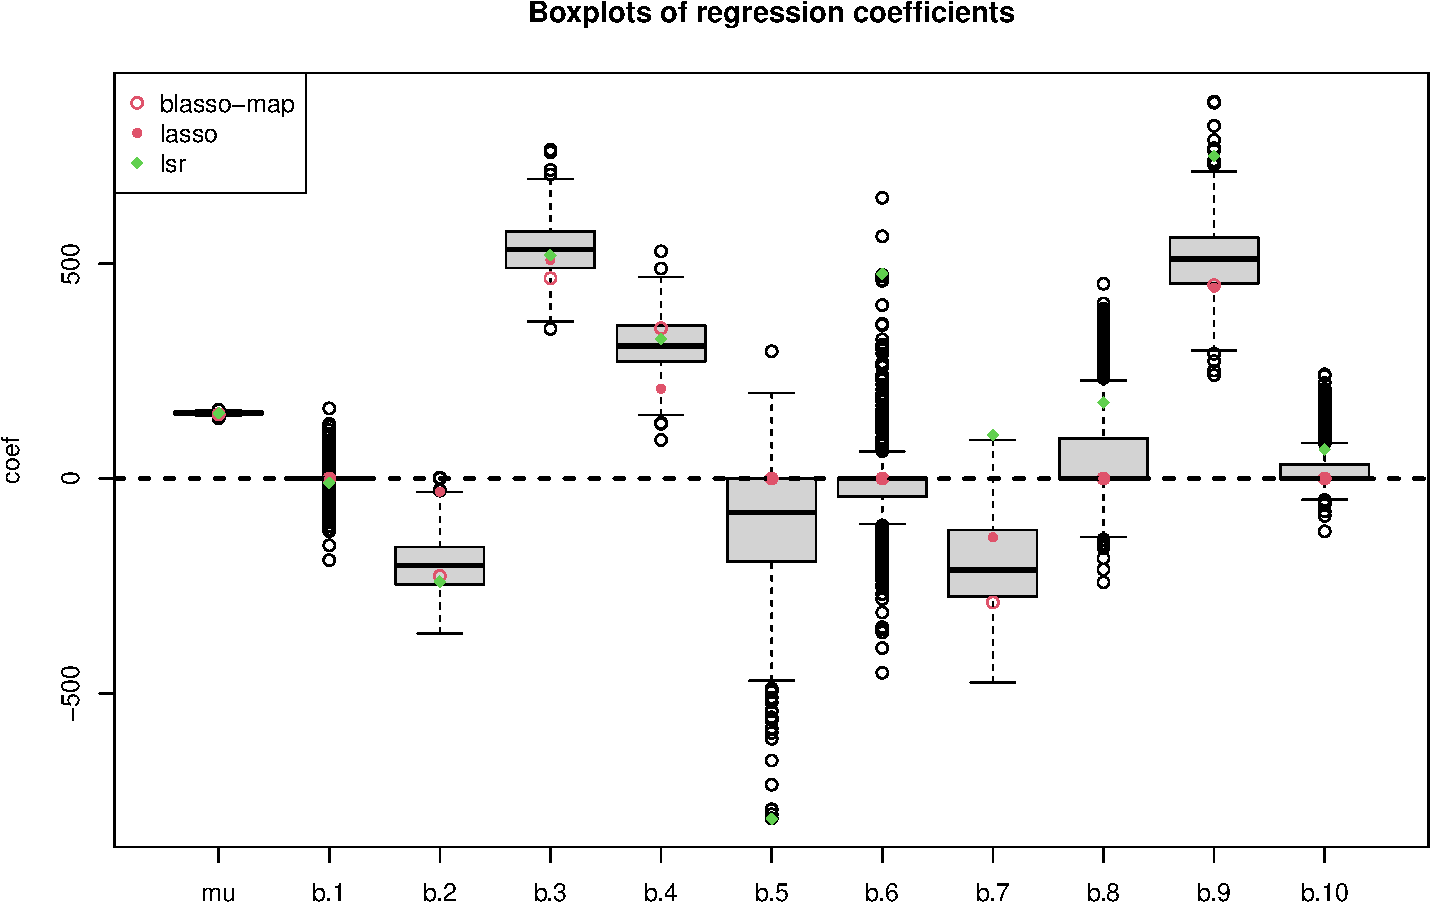
\includegraphics{L4_files/figure-beamer/unnamed-chunk-3-1.pdf}

\begin{Shaded}
\begin{Highlighting}[]
\CommentTok{## plot the size of different models visited}
\CommentTok{#plot(reg.blas, burnin=200, which="m")}

\CommentTok{## get the summary}
\NormalTok{s <-}\StringTok{ }\KeywordTok{summary}\NormalTok{(reg.blas, }\DataTypeTok{burnin=}\DecValTok{200}\NormalTok{)}

\CommentTok{## calculate the probability that each beta coef != zero}
\KeywordTok{barplot}\NormalTok{(s}\OperatorTok{$}\NormalTok{bn0,}\DataTypeTok{names.arg=}\KeywordTok{colnames}\NormalTok{(diabetes}\OperatorTok{$}\NormalTok{x),}\DataTypeTok{main=}\StringTok{"Probability each coefficient is NOT zero in the blasso"}\NormalTok{)}
\end{Highlighting}
\end{Shaded}

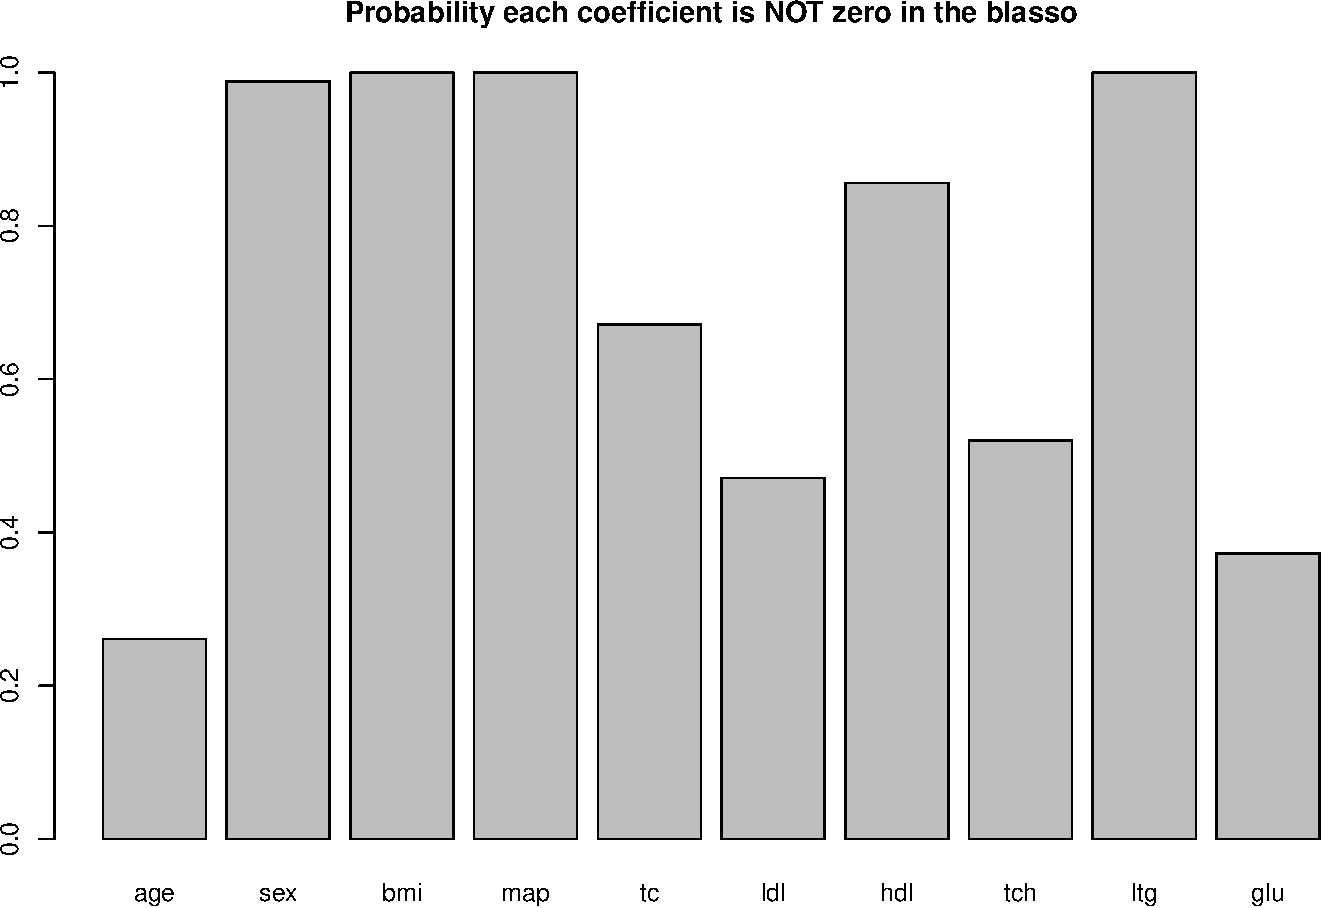
\includegraphics{L4_files/figure-beamer/unnamed-chunk-4-1.pdf}

\end{block}

\end{frame}

\begin{frame}{Bootstrap}
\protect\hypertarget{bootstrap}{}

(HTW 6.2)

\end{frame}

\begin{frame}

\begin{block}{Procedure to find lasso estimate
\(\hat{\beta}(\hat{\lambda}_{CV})\)}

(Copied word by word from HTW page 142)

Refer to these 6 steps as \(\hat{\beta}(\hat{\lambda}_{CV})\)-loop

\begin{enumerate}
\tightlist
\item
  Fit a lasso path to \((X, y)\) over a dense grid of values
  \(\Lambda=\{\lambda_l\}_{l=1}^{L}\).
\item
  Divide the training samples into 10 groups at random.
\item
  With the \(k\)th group left out, fit a lasso path to the remaining
  \(9/10\)ths, using the same grid \(\Lambda\).
\item
  For each \(\lambda \in \Lambda\) compute the mean-squared prediction
  error for the left-out group.
\item
  Average these errors to obtain a prediction error curve over the grid
  \(\Lambda\).
\item
  Find the value \(\hat{\beta}(\hat{\lambda}_{CV})\) that minimizes this
  curve, and then return the coefficient vector from our original fit in
  step (1) at that value of \(\lambda\).
\end{enumerate}

\end{block}

\end{frame}

\begin{frame}

\textbf{Observe:}

\begin{itemize}
\tightlist
\item
  \(\lambda\)-path is the same for each run of the lasso
\item
  the chosen \(\lambda\) is then used on the orginal data
\end{itemize}

\textbf{Q:} Is it possible to use resampling to estimate the
distribution of the lasso \(\hat{\beta}\) estimator including the model
selection (choosing \(\lambda\))?

\end{frame}

\begin{frame}

\begin{block}{Non-parametric (paired) bootstrap}

\begin{itemize}
\tightlist
\item
  Let \(F\) denote the joint distribution of \((X,Y)\).
\item
  The empirical \(\hat{F}\) is \(\frac{1}{N}\) for each observation
  \((X,Y)\) in our training data \((X_i,Y_i)\), \(i=1,\ldots,N\).
\item
  Drawing from \(\hat{F}\) is the same as drawing from the \(N\)
  observations in the training data with replacement.
\end{itemize}

Now, we draw \(B\) bootstrap samples from the training data, and for
each new bootstrap sample we run through the 6 steps in the
\(\hat{\beta}(\hat{\lambda}_{CV})\)-loop.

\begin{itemize}
\tightlist
\item
  The result is \(B\) vectors \(\hat{\beta}(\hat{\lambda}_{CV})\).
\item
  We plot the result as

  \begin{itemize}
  \tightlist
  \item
    boxplots,
  \item
    proportion of times each element of
    \(\hat{\beta}(\hat{\lambda}_{CV})\) is equal 0.
  \end{itemize}
\end{itemize}

\end{block}

\end{frame}

\begin{frame}

\begin{block}{Diabetes example}

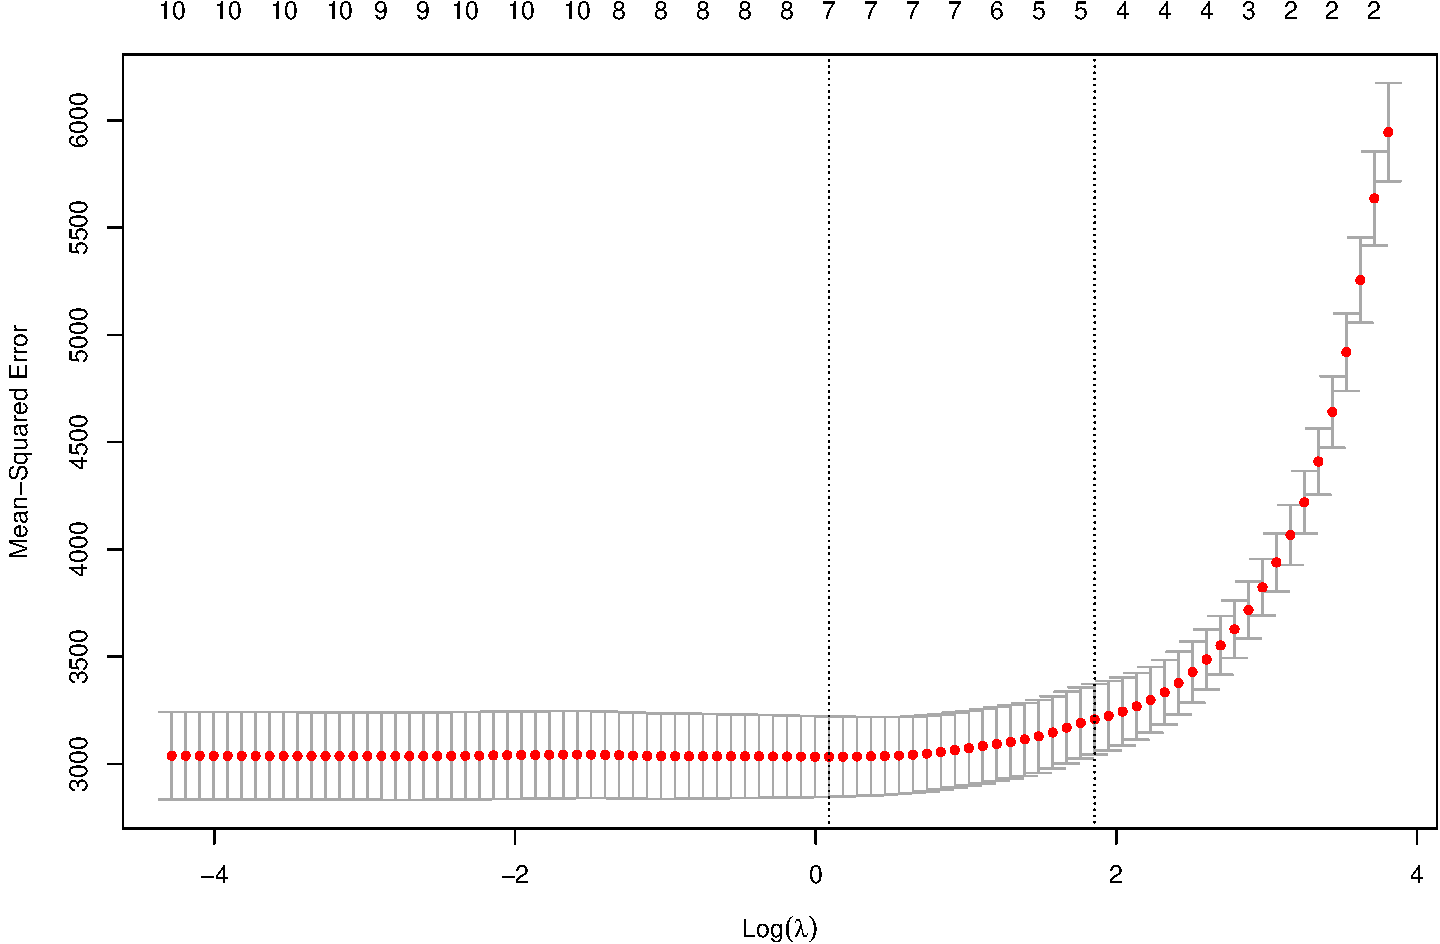
\includegraphics{L4_files/figure-beamer/unnamed-chunk-7-1.pdf}

\end{block}

\end{frame}

\begin{frame}

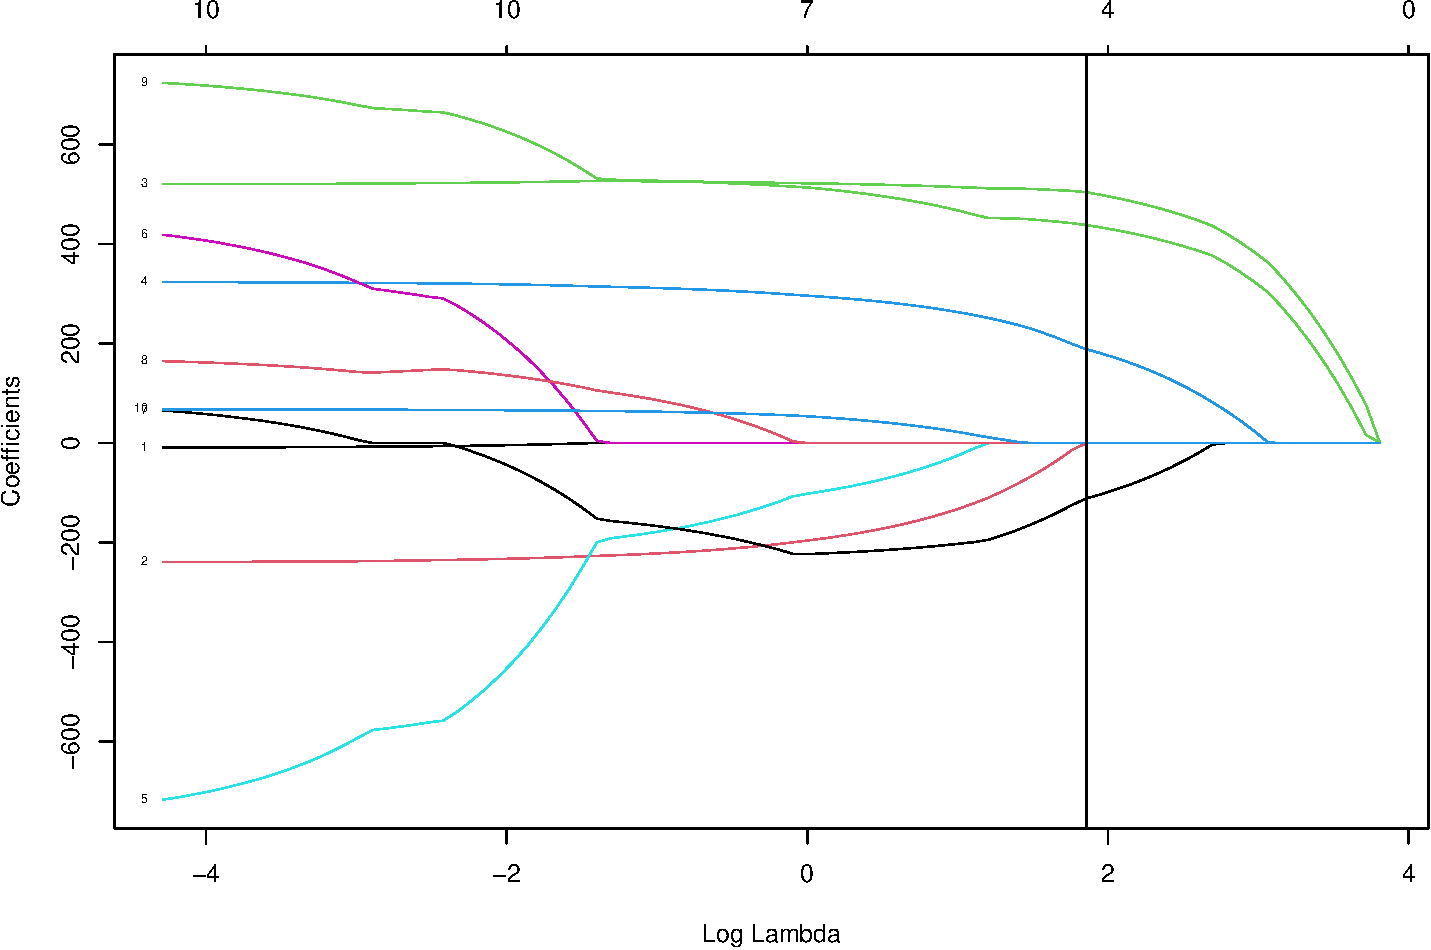
\includegraphics{L4_files/figure-beamer/unnamed-chunk-8-1.pdf}

\end{frame}

\begin{frame}[fragile]

\begin{verbatim}
## 11 x 1 sparse Matrix of class "dgCMatrix"
##                     1
## (Intercept)  152.1335
## age            .     
## sex            .     
## bmi          503.9260
## map          188.5872
## tc             .     
## ldl            .     
## hdl         -111.3725
## tch            .     
## ltg          438.1323
## glu            .
\end{verbatim}

\end{frame}

\begin{frame}[fragile]

\begin{Shaded}
\begin{Highlighting}[]
\NormalTok{lassomat=}\KeywordTok{dget}\NormalTok{(}\StringTok{"diabeteslassomat.dd"}\NormalTok{)}
\NormalTok{ridgemat=}\KeywordTok{dget}\NormalTok{(}\StringTok{"diabetesridgemat.dd"}\NormalTok{)}

\CommentTok{# plotting boxplots}

\NormalTok{lassomatUI=lassomat[,}\OperatorTok{-}\DecValTok{1}\NormalTok{]}
\NormalTok{lassods=reshape2}\OperatorTok{::}\KeywordTok{melt}\NormalTok{(lassomatUI,}
         \DataTypeTok{variable.name =}\StringTok{"variable"}\NormalTok{,}\DataTypeTok{value.name=}\StringTok{"value"}\NormalTok{)}
\NormalTok{lassopp=}\KeywordTok{ggplot}\NormalTok{(lassods,}\KeywordTok{aes}\NormalTok{(}\DataTypeTok{x=}\NormalTok{Var2,}\DataTypeTok{y=}\NormalTok{value))}\OperatorTok{+}\KeywordTok{geom_boxplot}\NormalTok{()}\OperatorTok{+}\KeywordTok{ggtitle}\NormalTok{(}\StringTok{"Boxplots for boostrapped lasso for diabetes data"}\NormalTok{)}
\NormalTok{lassopp}
\end{Highlighting}
\end{Shaded}

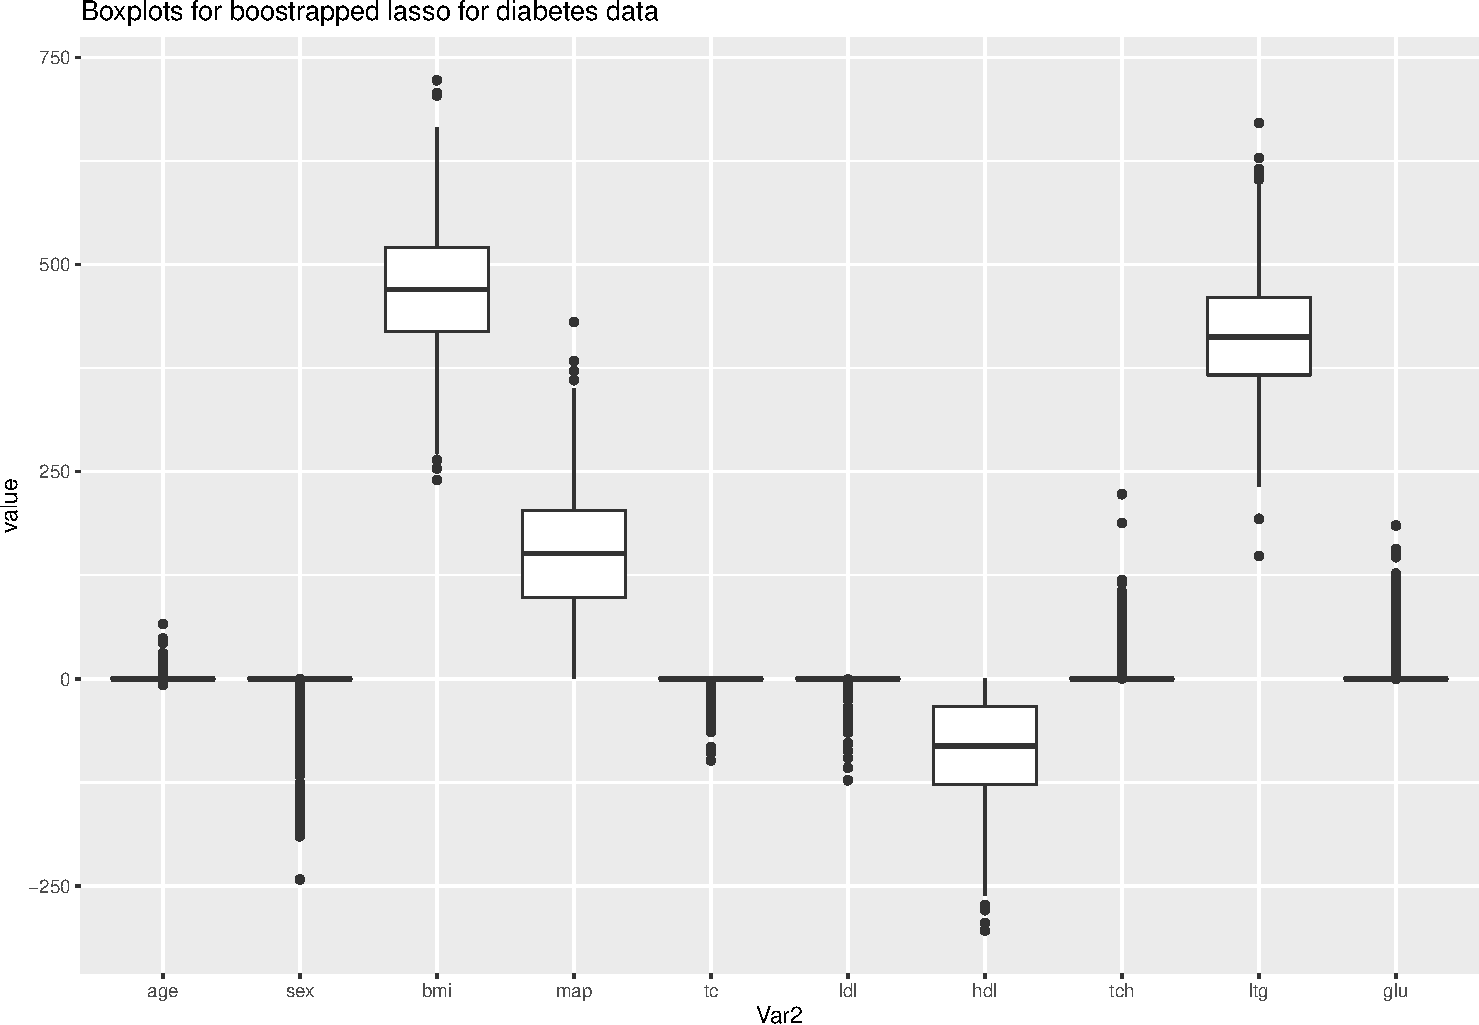
\includegraphics{L4_files/figure-beamer/unnamed-chunk-11-1.pdf}

\begin{Shaded}
\begin{Highlighting}[]
\NormalTok{ridgematUI=ridgemat[,}\OperatorTok{-}\DecValTok{1}\NormalTok{]}
\NormalTok{ridgeds=reshape2}\OperatorTok{::}\KeywordTok{melt}\NormalTok{(ridgematUI,}\DataTypeTok{variable.name=}\StringTok{"variable"}\NormalTok{,}\DataTypeTok{value.name=}\StringTok{"value"}\NormalTok{)}
\NormalTok{ridgepp=}\KeywordTok{ggplot}\NormalTok{(ridgeds,}\KeywordTok{aes}\NormalTok{(}\DataTypeTok{x=}\NormalTok{Var2,}\DataTypeTok{y=}\NormalTok{value))}\OperatorTok{+}\KeywordTok{geom_boxplot}\NormalTok{()}\OperatorTok{+}\KeywordTok{ggtitle}\NormalTok{(}\StringTok{"Boxplots for boostrapped ridge for diabetes data"}\NormalTok{)}
\NormalTok{ridgepp}
\end{Highlighting}
\end{Shaded}

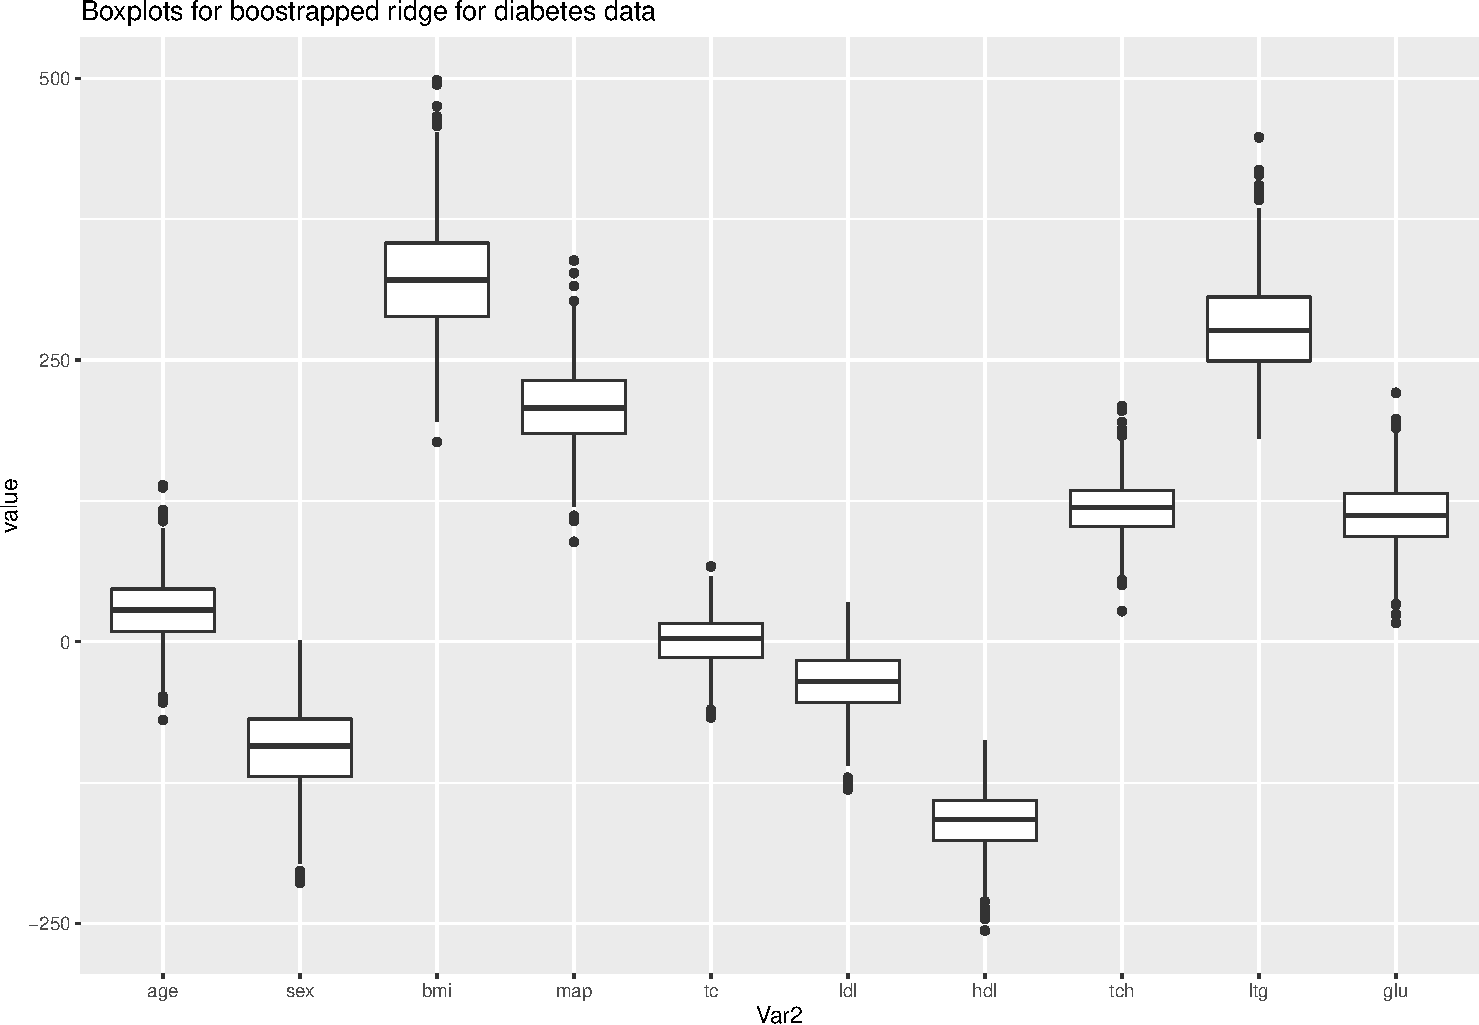
\includegraphics{L4_files/figure-beamer/unnamed-chunk-11-2.pdf}

\begin{Shaded}
\begin{Highlighting}[]
\NormalTok{lasso0perc=}\KeywordTok{apply}\NormalTok{(}\KeywordTok{abs}\NormalTok{(lassomat)}\OperatorTok{<}\NormalTok{.Machine}\OperatorTok{$}\NormalTok{double.eps,}\DecValTok{2}\NormalTok{,mean)}
\KeywordTok{barplot}\NormalTok{(lasso0perc)}
\end{Highlighting}
\end{Shaded}

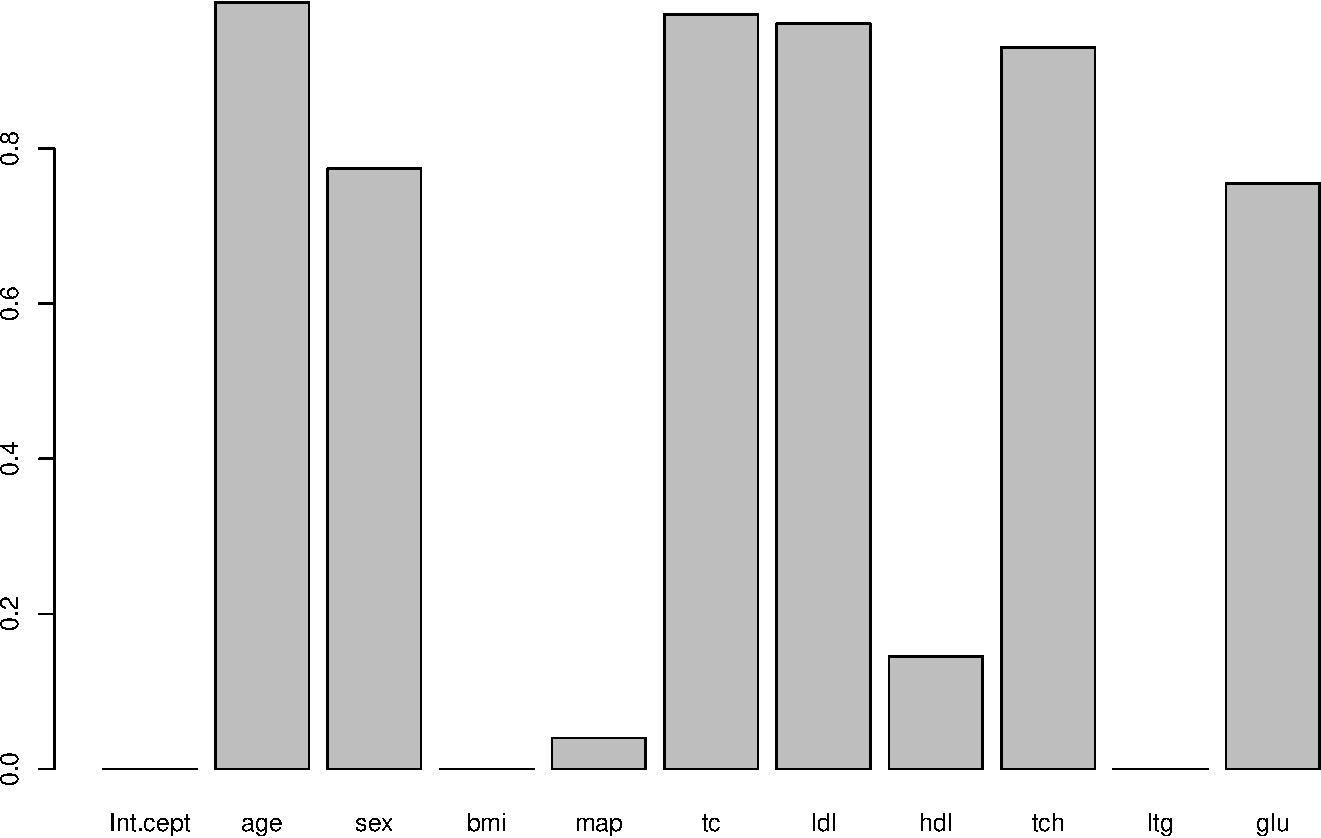
\includegraphics{L4_files/figure-beamer/unnamed-chunk-11-3.pdf}

\end{frame}

\begin{frame}

\begin{block}{Bootstrapping vs Bayesian lasso}

The results from the Bayesian lasso on the proportion of times a
coefficient is 0 and the boxplots are very similar to the results from
the bootstrapping. The bootstrap seems to be doing the ``same'' as a
Bayesian analysis with the Laplacian prior.

When the model is not so complex and the number of covariates is not too
large (\(p\sim 100\)) the Bayesian lasso might be as fast as the
bootstrapping, but for larger problems the bootstrap ``scales better''.

For GLMs the Bayesian solution is more demanding, but the bootstrap is
as easy as for the linear model.

(STudy and compare Figure 6.3 and 6.4 in HTW.)

\end{block}

\end{frame}

\begin{frame}

\begin{block}{Medical example}

(See Figures from study in slides.)

\end{block}

\end{frame}

\begin{frame}

\begin{block}{Bootstrap ridge and lasso percentile CI}

What if we calculated percentile bootstrap intervals - could we use that
to say anything about the true underlying regression coefficients?

\end{block}

\end{frame}

\begin{frame}

Sadly, there are two main challenges:

\begin{itemize}
\tightlist
\item
  The percentile interval is not a good choice for biased estimators.
\item
  It has been shown that (for fixed \(p\)) the asymptotic
  (\(n\leftarrow \infty\)) distribution of the lasso has point mass at
  zero (which leads to that bootstrapping not having optimal
  properties).
\end{itemize}

However: much research to check out here - with both different ways
perform the bootstrapping and different adjustments for the intervals!

One possibility is the R-package
\href{https://cran.r-project.org/web/packages/HDCI/HDCI.pdf}{HDCI} but
the background manuscript is not published yet
\url{https://arxiv.org/abs/1706.02150}.

\end{frame}

\begin{frame}{Sample splitting}
\protect\hypertarget{sample-splitting}{}

\begin{block}{What if we just split the data in two?}

Linear regression or logistic regression.

Dataset with \(p\) covariates and \(N\) observations. Divided into a
training set of size \(aN\) and a test set of \((1-a)N\), where
\(a \in [0,1]\).

\begin{itemize}
\item
  Training data used to decide on \(\lambda\) using CV - gives final
  model where some coefficients is set to 0 and some are shrunken. (The
  6 steps.)
\item
  Test data:

  \begin{itemize}
  \tightlist
  \item
    Fit ordinary LS or GLM model with only the non-zero lasso covariates
  \item
    present CI and \(p\)-values from LS
  \end{itemize}
\end{itemize}

\textbf{Group discussion:} Is this ok? What is gained and what is lost?

\end{block}

\end{frame}

\begin{frame}

\begin{block}{From single to multiple hypotheses}

In many situations we are not interested in testing only one hypothesis,
but instead \(m\) hypotheses.

\begin{longtable}[]{@{}llll@{}}
\toprule
& Not reject \(H_0\) & Reject \(H_0\) & Total\tabularnewline
\midrule
\endhead
\(H_0\) true & \(U\) & \(V\) & \(m_0\)\tabularnewline
\(H_0\) false & \(T\) & \(S\) & \(m - m_0\)\tabularnewline
Total & \(m-R\) & \(R\) & \(m\)\tabularnewline
\bottomrule
\end{longtable}

\begin{itemize}
\tightlist
\item
  Out of the \(m\) hypotheses tested, the (unknown) number of true null
  hypotheses is \(m_0\).
\item
  \(V\): the number of type I errors (false positive findings) and
\item
  \(T\): the number of type II errors (false negative findings).
\item
  \(U\): the number of true null hypotheses that are not rejected and
\item
  \(S\): the number of false null hypotheses that are rejected.
\item
  \(R\): the number of hypoteses rejected for a specific cut-off
\end{itemize}

Observe: only \(m\) and \(R\) is observed!

\end{block}

\end{frame}

\begin{frame}

\begin{block}{Familywise error rate}

The familywise error rate (FWER) is defined as \emph{the probability of
one or more false positive findings}

\[ \text{FWER} = P(V > 0) \] The number of false positive findings \(V\)
is not known in a real life situation, but still we may find a cut-off
on the \(p\)-value, called \(\alpha_{\text loc}\), that gives an upper
limit to (controls) the FWER.

\end{block}

\end{frame}

\begin{frame}

\begin{itemize}
\tightlist
\item
  Raw \(p\)-value, \(p_j\), the lowest nominal level to reject the null
  hypothesis.\\
\item
  Adjusted \(p\)-value, \(\tilde{p}_j\), is the nominal level of the
  multiple (simultaneous) test procedure at which
  \(H_{0j}, j=1,\ldots,m\) is just rejected, given the values of all
  test statistics involved.
\end{itemize}

The adjusted \(p\)-values can be defined as
\[\tilde{p}_j = \text{inf}\{\alpha  \mid H_{0j}\text{ is rejected at FWER level } \alpha \}\]

In a multiple testing problem where all adjusted \(p\)-value below
\(\alpha\) are rejected, the overall type I error rate (for example
FWER) will be controlled at level \(\alpha\).

\end{frame}

\begin{frame}

\begin{block}{The Bonferroni method controls the FWER}

Single-step methods controls for multiple testing by estimating one
local significance level, \(\alpha_{\text{loc}}\), which is used as a
cut-off to detect significance for each individual test.

The Bonferroni method is valid for all types of dependence structures
between the test statistics.

The local significance level is \[\alpha_{\text loc}=\frac{\alpha}{m}\]

The adjusted \(p\)-value is \[ \tilde{p}_j =\min(1,m p_j)\]

Read more here if needed:
\href{https://www.math.ntnu.no/emner/TMA4267/2017v/multtest.pdf}{Short
note on multiple hypothesis testing}

\end{block}

\end{frame}

\begin{frame}

\begin{block}{High-dimensional inference}

(Dezeure, Bühlmann, Meier, Meinshausen, 2.1.1 + 2.2)

\begin{itemize}
\tightlist
\item
  The article has focus on frequentist methods for high-dimensional
  inference with confidence intervals and \(p\)-values in linear and
  generalized linear models.
\item
  We will focus on linear models.
\end{itemize}

\end{block}

\end{frame}

\begin{frame}

\textbf{Set-up:}

\[Y={\bf X} \beta^0 +\varepsilon\]

\begin{itemize}
\tightlist
\item
  \({\bf X}\) is \(n\times p\) design matrix
\item
  \(Y\) is an \(n \times 1\) response vector
\item
  \(\varepsilon\) is an \(n \times 1\) error vector, independent of
  \({\bf X}\) and i.i.d. entries with \(\text{E}(\varepsilon)_i)=0\).
\item
  The number of parameters \emph{may} be larger than the sample size
  (then the regression parameter is not identifiable in general).
\end{itemize}

The \emph{active set} is \[S_0=\{ j; \beta_j^0 \neq 0,j=1,\ldots,p\}\]
with cardinality (size) \(\lvert S_0 \rvert\).

\textbf{Now:} construct CI and \(p\)-values for \emph{individual
regression parameters} \(\beta_j^0\), \(j=1,\ldots, p\), and also with
multiple testing adjustment.

Remark: We want inference for \emph{all} coefficients - not only the
ones that the lasso has selected.

\end{frame}

\begin{frame}

\begin{itemize}
\tightlist
\item
  The lasso has desirable properties for estimating \(\beta^0\) in high
  dimensional models, in particular for prediction \({\bf X}\beta^0\) or
  a new response \(Y_{\text{new}}\).
\item
  But, the distribution of the estimator is hard to characterize, and
\item
  it has been shown that (for fixed \(p\)) the asymptotic
  (\(n\leftarrow \infty\)) distribution of the lasso has point mass at
  zero (which leads to that bootstrapping not having optimal
  properties).
\end{itemize}

For the situation \(p >> n\) extra assumptions are needed, called the
\emph{compatibility condition} on the design matrix, and this guarantees
identifiability and socalled oracle optimality results for the lasso.
However, this is reported to be \emph{unrealistic in practical
situations}.

\end{frame}

\begin{frame}

\begin{block}{Single-sample splitting}

\begin{enumerate}
[1)]
\tightlist
\item
  Split the data into two (equal) halves, \(I_1\) and \(I_2\), no
  observations in common.
\item
  \(I_1\) is used for model selection (with the lasso), with active
  variables in \(\hat{S}(I_1)\).
\item
  The selected covariates in \(\hat{S}(I_1)\) is used for estimation in
  \(I_2\). To construct \(p\)-values, \(P_j\), for example use LS with
  \(t\)-tests. \(P\)-values for variables not selected is set to \(1\).
  Remark: then the number of covariates selected in \(I_1\) need be
  smaller than the sample size for \(I_2\).
\item
  The raw \(p\)-values is corrected for multiple testing (Bonferroni
  method controlling FWER)
  \[ P_{\text{corr},j}=\min(P_j \cdot \lvert \hat{S} \rvert,1)\]
\end{enumerate}

This avoids using the data twice! But, is very sensitive to the split -
giving \emph{wildly} different \(p\)-values=\emph{\(p\)-value lottery}

How can this be amended?

\end{block}

\end{frame}

\begin{frame}

\begin{block}{Multiple-sample splitting}

\begin{itemize}
\item
  The single-sample splitting routine is run \(B\) times giving
  \(P_{\text{corr},j}^{[b]}\) for \(b=1,\ldots,B\) and \(j=1,\ldots,p\).
\item
  Problem: how aggregate the \(B\) \(p\)-values for each \(j\) to give
  one \(p\)-value?
\item
  The different \(b\) runs have many observations in common, so the
  \(p\)-values for covariate \(j\) are correlated.
\item
  The authors have shown in a previous article that for dependent
  \(p\)-values that one solution (that gives valid \(p\)-values) is to
  take the median and multiply with 2.
\item
  The result is more general, and \(\gamma\) is a general quantile
  (\(\gamma=0.5\) for the median):
\end{itemize}

\[Q_k(\gamma)=\min(\text{empirical }\gamma- \text{quantile} \{ P_{\text{corr},j}^{[b]}/\gamma,b=1,\ldots, B\},1)\]

\end{block}

\end{frame}

\begin{frame}

\begin{itemize}
\tightlist
\item
  The authors get more advanced and choose to search all \(\gamma\)
  within the interval \((\gamma_{\text{min}},1)\), where a common choice
  is \(\gamma_{\text{min}}=0.05\), to get the smallest \(p\)-value.
  However there is a price to pay: \((1-\log(\gamma_{\text{min}}))\)
\end{itemize}

\[ P_j=\min((1-\log(\gamma_{\text{min}})\cdot \inf_{\gamma \in (\gamma_{\text{min}},1)} Q_j(\gamma)),1)\]
for \(j=1,\ldots,p\).

Some assumptions are necessary to assure FWER control.

\end{frame}

\begin{frame}

Confidence intervals are found

\begin{itemize}
\tightlist
\item
  from the adjusted \(p\)-values \(P_j\)
\item
  using the duality of \(p\)-values and two-sided confidence intervals.
  That is,
\item
  a \((1-\alpha)\) 100\% CI contains values \(c\) where the \(p\)-value
  is below \(\alpha\) for testing \(H_0: \beta_j=c\). A closed form
  solution involving \(P_j\) is found.
\item
  Both single testing and multiple corrected testing CIs are found.
  (Appendix A.2 in article)
\end{itemize}

\end{frame}

\begin{frame}[fragile]

\footnotesize

\begin{Shaded}
\begin{Highlighting}[]
\KeywordTok{data}\NormalTok{(diabetes)}
\NormalTok{x=}\KeywordTok{cbind}\NormalTok{(diabetes}\OperatorTok{$}\NormalTok{x)}\CommentTok{#,diabetes$x2)}
\NormalTok{y=diabetes}\OperatorTok{$}\NormalTok{y}

\NormalTok{hdires=}\KeywordTok{multi.split}\NormalTok{(}\DataTypeTok{x=}\NormalTok{x,}\DataTypeTok{y=}\NormalTok{y,}\DataTypeTok{B=}\DecValTok{1000}\NormalTok{,}\DataTypeTok{fraction=}\FloatTok{0.5}\NormalTok{,}
                   \DataTypeTok{ci.level=}\FloatTok{0.95}\NormalTok{, }\DataTypeTok{model.selector=}\NormalTok{lasso.cv,}
                   \DataTypeTok{classical.fit=}\NormalTok{lm.pval, }\DataTypeTok{classical.ci=}\NormalTok{lm.ci,}
                   \DataTypeTok{return.nonaggr =} \OtherTok{FALSE}\NormalTok{, }\CommentTok{#if not adj for multiple testing}
                   \DataTypeTok{return.selmodels=}\OtherTok{FALSE}\NormalTok{, }\CommentTok{#just to have a look!}
                   \DataTypeTok{verbose=}\OtherTok{FALSE}\NormalTok{)}
\KeywordTok{dput}\NormalTok{(hdires,}\StringTok{"hdires.dd"}\NormalTok{)}
\end{Highlighting}
\end{Shaded}

\end{frame}

\begin{frame}[fragile]

\begin{Shaded}
\begin{Highlighting}[]
\NormalTok{hdires=}\KeywordTok{dget}\NormalTok{(}\StringTok{"hdires.dd"}\NormalTok{)}
\KeywordTok{names}\NormalTok{(hdires)}
\end{Highlighting}
\end{Shaded}

\begin{verbatim}
##  [1] "pval"             "pval.corr"        "pvals.nonaggr"    "ci.level"        
##  [5] "lci"              "uci"              "gamma.min"        "sel.models"      
##  [9] "method"           "call"             "clusterGroupTest"
\end{verbatim}

\begin{Shaded}
\begin{Highlighting}[]
\NormalTok{hdires}\OperatorTok{$}\NormalTok{gamma.min}
\end{Highlighting}
\end{Shaded}

\begin{verbatim}
##  [1] 0.999 0.999 0.050 0.064 0.999 0.999 0.050 0.999 0.052 0.999
\end{verbatim}

\begin{Shaded}
\begin{Highlighting}[]
\CommentTok{#summary(hdires$pvals.nonaggr) # if return.nonaggr=TRUE}
\NormalTok{hdires}\OperatorTok{$}\NormalTok{pval.corr}
\end{Highlighting}
\end{Shaded}

\begin{verbatim}
##          age          sex          bmi          map           tc          ldl 
## 1.000000e+00 1.000000e+00 5.178832e-10 1.331537e-02 1.000000e+00 1.000000e+00 
##          hdl          tch          ltg          glu 
## 4.533731e-01 1.000000e+00 6.863052e-08 1.000000e+00
\end{verbatim}

\begin{Shaded}
\begin{Highlighting}[]
\KeywordTok{cbind}\NormalTok{(hdires}\OperatorTok{$}\NormalTok{lci, hdires}\OperatorTok{$}\NormalTok{uci)}
\end{Highlighting}
\end{Shaded}

\begin{verbatim}
##           [,1]      [,2]
## age       -Inf       Inf
## sex -435.92911 103.48598
## bmi  363.10330 776.42063
## map   66.58321 472.64439
## tc        -Inf       Inf
## ldl       -Inf       Inf
## hdl -406.96777  14.72096
## tch -764.32633 201.01275
## ltg  301.70828 715.18364
## glu -327.08642 254.88420
\end{verbatim}

\normalsize

\end{frame}

\begin{frame}[fragile]

\begin{block}{hdi with logistic regression}

For modifications to the call to \texttt{mult.split} see the Appendix of
the master thesis of

\begin{itemize}
\tightlist
\item
  Martina Hall: \href{http://hdl.handle.net/11250/2453095}{``Statistical
  Methods for early Prediction of Cerebral Palsy based on Data from
  Computer-based Video Analysis''}.
\item
  Dag J. Kristiansen:
  \href{http://hdl.handle.net/11250/2624609}{``Detecting Neuronal
  Activity with Lasso Penalized Logistic Regression''}
\item
  Haris Fawad: " Modelling Neuronal Activity using Lasso Regularized
  Logistic Regression"( Modelling Neuronal Activity using Lasso
  Regularized Logistic Regression) - also
  \href{https://github.com/harisf/neuro-lasso}{git repo neuro-lasso}.
\end{itemize}

\end{block}

\begin{block}{hdi - also with other solutions}

In the \texttt{hdi} package also solutions for \emph{debiasing} the
lasso estimator is included. (See HTW 6.4 or the Dezure et al article.)

\end{block}

\end{frame}

\begin{frame}

\begin{block}{Summing up}

What is the take home message from this ``Sample splitting'' story?

\end{block}

\end{frame}

\begin{frame}{Inference after selection}
\protect\hypertarget{inference-after-selection}{}

(Taylor and Tibshirani, 2015 and HTW 6.3)

\begin{block}{The plot}

Let us leave the lasso for a while.

1980: small data sets, planned hypothesis to test ready before data
collected, no model selection. Only fit model and look at CI and
p-values.

After 1980: larger data sets and looking at data to give best model. New
challenge: \emph{how to do inference after selection}.

This is an important topic that is not a part of ANY statistical courses
at IMF.

The main question is:

\begin{itemize}
\tightlist
\item
  we have used a selection method (forward selection, lasso) to find
  potential association between covariates and response,
\item
  with focus on interpreting the selected model: how can we assess the
  strength (read: CI and \(p\)-value) of these findings?
\end{itemize}

\end{block}

\end{frame}

\begin{frame}

The answer includes:

\begin{itemize}
\tightlist
\item
  we have ``cherry picked'' the strongest associations, and we can thus
  not just report CI and \(p\)-values based on the final model - when
  all is done on the same data set.
\end{itemize}

In this story we now focus on \emph{understanding how our model
selection influences the inference on the final model}.

The technical solutions are of less importance, and is not presented
with enough mathematical detail so that we understand the method in
detail.

\emph{Remark: the single and multiple sample splitting strategy
isvalid.}

\end{frame}

\begin{frame}

\begin{block}{Forward stepwise regression}

\textbf{Aim:} Multiple linear regression - where forward stepwise
regression is used to select the model

\[y_i=\beta_0+\sum_{j=1}^p x_{ij}\beta_j + \varepsilon_i\]

\begin{itemize}
\tightlist
\item
  Start with an empty model (only intercept)
\end{itemize}

While some stopping criterion not reach - perform step

\begin{itemize}
\tightlist
\item
  At step \(k\) add the predictor that gives the most decrease in the
  sums of squares of error (here now - to follow the notation denoted by
  RSS instead of what we previously called SSE)
\end{itemize}

\[ \text{RSS}=\sum_{i=1}^N (y_i -\hat{y}_i)^2\] where \(\hat{y}_i\) is
the predicted value for observation \(i\) in this model.

\end{block}

\end{frame}

\begin{frame}

If we have a model with \(k-1\) predictors and we would like to add one
more predictor (the \(k\) to be added):

\[ \text{R}_k=\frac{1}{\sigma^2}(\text{RSS}_{k-1}-\text{RSS}_{k})\sim \chi^2_1\]
where here \(\sigma^2\) is assumed known.

This can be seen as an hypothesis test:

\(H_0: \text{The new predictor is not relevant}\)
vs.~\(H_1: \text{The new predictor is relevant}\) with a \(p\)-value
calculated from the upper tail of the \(\chi^2_1\)-distribution.

\end{frame}

\begin{frame}

\textbf{Alternative scenario: }

For simplicity - we look at the \(k=1\):

The order in which the predictors is to be entered in to the model was
decided before the data was collected (or at least before the data was
analysed or plottet).

Then: we are all good - and this \(p\)-value from the
\(\chi^2_1\)-distribution will be a valid \(p\)-value.

What does this mean in practice?

\end{frame}

\begin{frame}

\textbf{Back to original scenario:}

Assume we are at step \(k=1\), and will add the first predictor which is
the one with the largest \(R_1\).

Will the distribution of the \emph{maximal} \(R_1\) be the same as the
distribution of a given predefined \(R_1\)?

Distribution to the maximum given that we have \(p\) predictors:

\[ P(\max R_1 \ge c)=1-P(\max R_1 < c)=1-P(\text{all p } R_1 \text{ are} <c)\]

Study Figure 1 in the article for a plot of nominal vs.~actual
\(p\)-value for \(p=10\) and \(p=50\). The figure was made using Monte
Carlo sampling.

\end{frame}

\begin{frame}

\textbf{Moving on to \(k>1\)}

\begin{itemize}
\tightlist
\item
  We would like to obtain valid (``correct'') \(p\)-values for all
  steps, not only for \(k=1\).
\item
  Monte Carlo solution would be elaborate.
\end{itemize}

The method used in the article is to calculate a \(p\)-value for the
covariate at step \(k\) by conditioning on the fact that already the
strongest \(k-1\) predictors in this sequential set-up has already been
chosen.

The \(p\)-value at step \(k\) would be dependent on the number of
covariates \(p\).

We now change focus and look at the distribution of the estimated
regression coefficient for the covariate added at step \(k\), because
that can be used to construct both a CI for the coefficient and a
\(p\)-value for testing if the coefficient is different from zero.

\end{frame}

\begin{frame}

\begin{block}{The polyhedral result}

(for details consult HTW 6.3 or articles references to in the Taylor and
Tibshirani article)

\textbf{Distribution for regression coefficient:}

\begin{itemize}
\tightlist
\item
  Assume that we are at some step \(k\), and that \(k-1\) covariates are
  in the model.
\item
  We have found the new covariate to include, and fitted the model with
  the \(k\) covariates.
\item
  Standard theory tells us that the estimator \(\hat{\beta}\) for
  covariate \(k\) is unbiased and follows a normal distribution with
  some variance \(\tau^2\).
\end{itemize}

\[ \hat{\beta} \sim N(\beta,\tau^2)\]

\end{block}

\end{frame}

\begin{frame}

But, this is given that we only had these \(k\) covariates available at
the start. We will instead \emph{condition on} selection event.

It turns out that the selection event can be written in a
\emph{polyhedral form} \(A y \le b\) for some matrix \(A\) and some
vector \(b\).

At each step of the forward selection we have a competition among all
\(p\) variables, and the \(A\) and \(b\) is used to construct the
competition.

\end{frame}

\begin{frame}

The correct distribution of the estimator \(\hat{\beta}\) for covariate
now has a \emph{truncated normal distribution}

\[ \hat{\beta} \sim TN^{c,d}(\beta,\tau^2)\]

i.e.~the \emph{same} normal distribution, but scaled to lie within the
interval \((c,d)\).

The limits \((c,d)\) depends on both the data and the selection evetns
that lead to the current model.

\emph{The formulae for these limits are somewhat complicated but easily
computable}.

This truncated normal distribution is used to calculate
\emph{selection-adjusted} \(p\)-values and confidence interval.

(Study Figure 3. in the article by Taylor and Tibshirani.)

\end{frame}

\begin{frame}

\begin{block}{Polythedral lasso result}

The same methodology can be used for the lasso, here also the selection
of predictors can be described as a polythedral region of the form
\(Ay\le b\) - for a fixed value \(\lambda\).

For the lass the \(A\) and \(b\) will depend on

\begin{itemize}
\tightlist
\item
  the predictors
\item
  the active set
\item
  \(\lambda\)
\end{itemize}

but not on \(y\).

The methods are on closed form, but the values \(c\) and \(d\) may be of
complicated form.

\end{block}

\end{frame}

\begin{frame}[fragile]

The R package \texttt{selectiveInference} can be used to find post
selection \(p\)-values both for forward stepwise selection and for the
lasso.

See the package help for details.

Study Figure 5 from the article for an example of Naive and
Selection-adjusted intervals for the lasso.

\end{frame}

\begin{frame}

\begin{block}{Further improvements}

The method yields rather wide confidence intervals for the regression
parameters (given that we translate the \(p\)-values into CIs).

There exists improvements to the results, in particular a method called
\emph{carving} which is explained in the you-tube videos from a course
with
\href{https://lsa.umich.edu/stats/people/faculty/psnigdha.html}{Snigdha
Paragrahi}

\begin{itemize}
\tightlist
\item
  \href{https://www.youtube.com/watch?v=qofrkW-DL7c\&t=3682s}{Tutorial
  I}
\item
  \href{https://www.youtube.com/watch?v=rGHf6BPeqBg\&t=1105s}{Tutorial
  II}
\end{itemize}

\end{block}

\end{frame}

\begin{frame}

\begin{block}{PoSI}

(HTW 6.5)

\begin{itemize}
\tightlist
\item
  The POSI method also fits a selected submodel and
\item
  adjust the standard CIs by \emph{accounting for all possible models
  that might have been delivered by the selection procedure}.
\item
  This means the method can be used on published results where the
  complete selection process is not explained in detail.
\item
  This lack of information of the selection process leads to \emph{very
  wide CIs}.
\end{itemize}

Inference is based on the submodel \(M\) chosen, and on the projection
of \({\bf X} \beta\) onto the space spanned by the submodel \(M\):

\[\beta_M=({\bf X}_M^T{\bf X}_M)^{-1}{\bf X}_M^T{\bf X} \beta\]

\end{block}

\end{frame}

\begin{frame}

The method considers a confidence interval for the \(j\)th element of
\(\beta_M\) of the form
\[\text{CI}_{jM}=\hat{\beta}_{jM}\pm K \hat{\sigma}v_{jM}\] where
\(v_{jM}^2=({\bf X}_M^T{\bf X}_M)^{-1}_{jj}\)

The constant \(K\) is found to satisfy
\[ P(\beta_{jM}\in \text{CI}_{jM}) \le 1-2\alpha\] \emph{over all
possible selection models}.

\end{frame}

\begin{frame}

\(K\) is a function of the data matrix \({\bf X}\) and the maximum
number of nonzero component allowed in \(\beta_M\). An upper bound on
\(K\) is known from a result on simultaneous intervals by Scheffe.

HTW page 161: Reports on the diabetes data with submodels of size 5,
where the 95\% CI value of K is 4.42 (``little less than 2 hours of
computing'').

Details may be found in the PoSI 2013 article (reference Berk et al
below).

\end{frame}

\begin{frame}

\begin{block}{PoSI R-package}

\emph{In linear LS regression, calculate for a given design matrix the
multiplier \(K\) of coefficient standard errors such that the confidence
intervals {[}b - K\emph{SE(b), b + K}SE(b){]} have a guaranteed coverage
probability for all coefficient estimates b in any submodels after
performing arbitrary model selection.}

Results for the Boston housing data is available in the help section.

\url{https://cran.r-project.org/web/packages/PoSI/index.html}

\end{block}

\end{frame}

\begin{frame}

\begin{block}{Post selection inference and the reproducibility crisis}

The \emph{incorrect} use of CIs and \(p\)-values in models found from
model selection \emph{and} inference on the same data - is though to be
one of the main contributors to the \emph{reproducibility crisis in
science}.

\href{https://hdsr.mitpress.mit.edu/pub/l39rpgyc/release/1}{Selective
Inference: The Silent Killer of Replicability by Yoav Benjamini
Published on Dec 16, 2020}

\end{block}

\end{frame}

\begin{frame}{Conclusion}
\protect\hypertarget{conclusion-1}{}

\begin{block}{How will you perform inference}

on Data Analysis Project 1?

We discuss:

\begin{enumerate}
[1)]
\tightlist
\item
  You can afford a test set
\item
  You have no test set
\end{enumerate}

\end{block}

\end{frame}

\begin{frame}{References}
\protect\hypertarget{references}{}

(also given in the text and not repeated here)

\begin{itemize}
\tightlist
\item
  \href{https://arxiv.org/pdf/1509.09169.pdf}{Wessel N. van Wieringen:
  Lecture notes on ridge regression}
\item
  A. Chatterjee and S. N. Lahiri (2011). Bootstrapping Lasso Estimators.
  Journal of the American Statistical Association. Vol. 106, No.~494
  (June 2011), pp.~608-625 (18 pages)
\item
  Single/multi-sampling splitting part of
  \href{https://projecteuclid.org/download/pdfview_1/euclid.ss/1449670857}{Dezeure,
  Bühlmann, Meier, Meinshausen (2015)}. ``High-Dimensional Inference:
  Confidence Intervals, p-Values and R-Software hdi''. Statistical
  Science, 2015, Vol. 30, No.~4, 533--558 DOI: 10.1214/15-STS527 (only
  the single/multiple sample splitting part in 2.1.1 and 2.2 for linear
  regression, and using the method in practice).
\item
  \href{https://www.pnas.org/content/112/25/7629}{Taylor and Tibshirani
  (2015)}: Statistical learning and selective inference, PNAS, vol 112,
  no 25, pages 7629-7634. (Soft version of HTW 6.3.2)
\item
  Berk, Richard; Brown, Lawrence; Buja, Andreas; Zhang, Kai; Zhao,
  Linda. Valid post-selection inference. Ann. Statist. 41 (2013), no. 2,
  802--837. \url{doi:10.1214/12-AOS1077}.
\end{itemize}

\end{frame}

\end{document}
